\documentclass[a4paper,12pt]{report}

\usepackage{cmap}
\usepackage[T2A]{fontenc}
\usepackage[utf8]{inputenc}
\usepackage[english,russian]{babel}
\usepackage{listings}
\usepackage{amsmath}
\usepackage{float}
\usepackage{csquotes}
\usepackage{mathtools}
\usepackage{hyphenat}
\usepackage{amsfonts}
\usepackage{upgreek}

\usepackage{xcolor}
\usepackage{hyperref}

\usepackage{graphicx}
\graphicspath{ {./img/} }

\definecolor{dkgreen}{rgb}{0,0.6,0}
\definecolor{gray}{rgb}{0.5,0.5,0.5}
\definecolor{mauve}{rgb}{0.58,0,0.82}

\lstset{
    language=Python,               
    basicstyle=\small\sffamily,
    numbers=left,              
    numberstyle=\tiny,         
    stepnumber=1,                 
    numbersep=5pt,              
    aboveskip=3mm,
    belowskip=3mm,
    showstringspaces=false,
    columns=flexible,
    captionpos=b, 
    basicstyle={\small\ttfamily},
    numbers=left,
    numberstyle=\tiny\color{gray},
    keywordstyle=\color{blue},
    commentstyle=\color{mauve},
    stringstyle=\color{dkgreen},
    breaklines=true,
    breakatwhitespace=true,
    tabsize=3
}

\title{Лабораторная работа №9\\Дифференцирование и интегрирование}
\author{Смирнов Никита}
\date{\today}

\begin{document}

\maketitle
\tableofcontents
\listoffigures
\lstlistoflistings

\maketitle

\chapter{Упражнение 9.1}

В данном упражнении нам нужно открыть \texttt{chap09.ipynb}, прочитать пояснения и  запустить примеры. Поэтому я просто изучил все примеры с комментариями.
\chapter{Упражнение 9.2}

Создаю треугольный сигнал \texttt{TriangleSignal}:

\begin{lstlisting}[caption=Создание треугольного сигнала]
in_wave = thinkdsp.TriangleSignal(freq=30).make_wave(duration=0.1, framerate=44100)
in_wave.plot()
thinkplot.config(xlabel='Time (s)')
\end{lstlisting}

\begin{figure}[H]
        \centering
        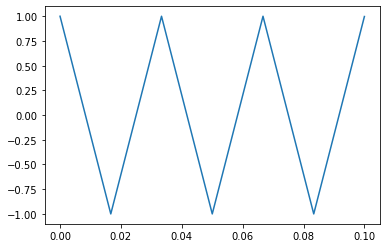
\includegraphics[width=0.75\textwidth]{1.png}
        \caption{Треугольный сигнал}
        \label{1}
\end{figure}

Применяю\texttt{diff}. \texttt{diff} от треугольной функции - прямоугольная функция. Можно сказать, что гармнрнтки прямоугльной и треугольной гармоники совпадают по $1/f$ и $1/f2$.



\begin{lstlisting}[caption=Визуализация при \texttt{diff}]
out_wave = in_wave.diff()
out_wave.plot()
\end{lstlisting}

\begin{figure}[H]
        \centering
        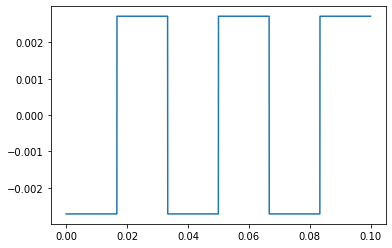
\includegraphics[width=0.75\textwidth]{2.png}
        \caption{Визуализация при использовании\texttt{diff}}
        \label{2}
\end{figure}

Когда мы берём спектральную производную, мы получаем "звон" вокруг разрывов.

\begin{lstlisting}[caption=Визуализация при \texttt{differentiate}]
out_wave2 = in_wave.make_spectrum().differentiate().make_wave()
out_wave2.plot()
\end{lstlisting}

\begin{figure}[H]
        \centering
        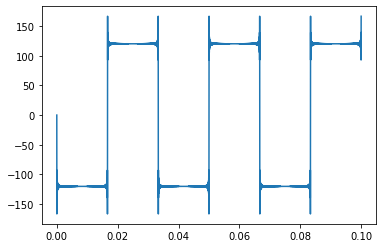
\includegraphics[width=0.75\textwidth]{3.png}
        \caption{Визуализация при использовании\texttt{differentiate}}
        \label{3}
\end{figure}

Различия между \texttt{diff} и \texttt{differentiate} заключается в том, что производная треугольной волны не определена в точках треугольника.

\chapter{Упражнение 9.3}

Для начала я создал прямоугольный сигнал.

\begin{lstlisting}[caption=Создание сигнала]
in_wave = thinkdsp.SquareSignal(freq=30).make_wave(duration=0.1, framerate=44100)
in_wave.plot()
\end{lstlisting}

\begin{figure}[H]
        \centering
        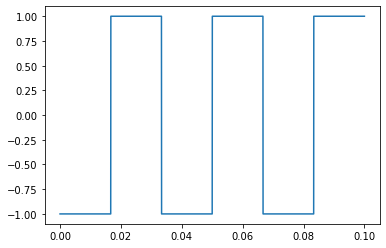
\includegraphics[width=0.75\textwidth]{4.png}
        \caption{Прямоугольный сигнал}
        \label{4}
\end{figure}

Мы получим треугольный сигнал из прямоугольного, что довольно логично после выполнения предыдущего упражнения.

\begin{lstlisting}[caption=Визуализация при \texttt{cumsum}]
out_wave = in_wave.cumsum()
out_wave.plot()
thinkplot.config(xlabel='Time (s)')
\end{lstlisting}

\begin{figure}[H]
        \centering
        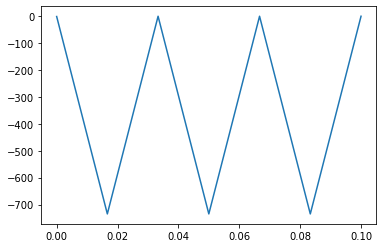
\includegraphics[width=0.75\textwidth]{5.png}
        \caption{Визуализация при использовании\texttt{cumsum}}
        \label{5}
\end{figure}

Создаем спектр сигнала и используем фйнкцию \texttt{integrate} и получаем новый сигнал на его основе.

\begin{lstlisting}[caption=Визуализация при \texttt{integrate}]
spectrum = in_wave.make_spectrum().integrate()
spectrum.hs[0] = 0
out_wave2 = spectrum.make_wave()
out_wave2.plot()
\end{lstlisting}

\begin{figure}[H]
        \centering
        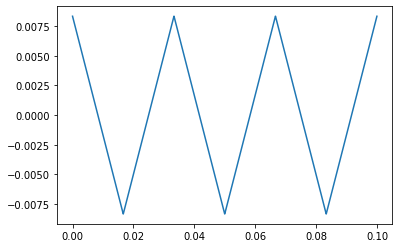
\includegraphics[width=0.75\textwidth]{6.png}
        \caption{Визуализация при использовании\texttt{integrate}}
        \label{6}
\end{figure}

Если уравновесить и нормализовать две волны, они будут визуально похожи.

\begin{lstlisting}[caption=Сравнение волн]
out_wave.unbias()
out_wave.normalize()
out_wave2.normalize()
out_wave.plot()
out_wave2.plot()
\end{lstlisting}

\begin{figure}[H]
        \centering
        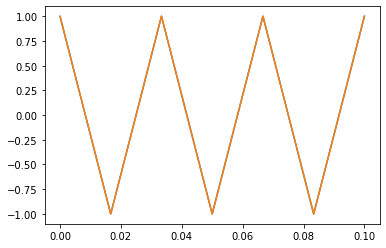
\includegraphics[width=0.75\textwidth]{7.png}
        \caption{Сравнение волн}
        \label{7}
\end{figure}

\begin{lstlisting}[caption=Разница между реализациями]
max(abs(out_wave.ys - out_wave2.ys))
\end{lstlisting}

Считаем разницу между реализациями и получаем \texttt{0.0027210884353741083}.

\chapter{Упражнение 9.4}

Создаю пилообразный сигнал.

\begin{lstlisting}[caption=Создание сигнала]
in_wave = thinkdsp.SawtoothSignal(freq=30).make_wave(duration=0.1, framerate=44100)
in_wave.plot()
\end{lstlisting}

\begin{figure}[H]
        \centering
        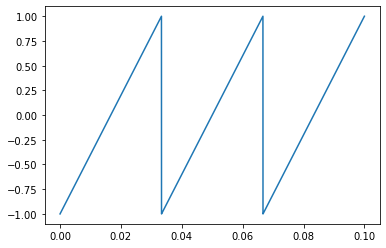
\includegraphics[width=0.75\textwidth]{8.png}
        \caption{Создание сигнала}
        \label{8}
\end{figure}

Вычисляем спектр и применяем к нему функцию \texttt{integrate} два раза.

\begin{lstlisting}[caption=двойное применение \texttt{integrate}]
out_wave = in_wave.cumsum()
out_wave.unbias()
out_wave.plot()
out_wave = in_wave.cumsum()
out_wave.unbias()
out_wave.plot()
\end{lstlisting}

\begin{figure}[H]
        \centering
        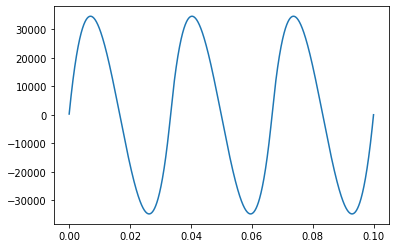
\includegraphics[width=0.75\textwidth]{9.png}
        \caption{Двойное применение \texttt{integrate}}
        \label{9}
\end{figure}

Двойное интегрирование дает кубическую кривую. На этом этапе результат всё больше и больше напоминает синусоиду. Причина в том, что интеграция действует как фильтр нижних частот. 

\chapter{Упражнение 9.5}

Создадим кубически   сигнал.

\begin{lstlisting}[caption=Создание сигнала]
in_wave = thinkdsp.CubicSignal(freq=0.0005).make_wave(duration=10000, framerate=1)
in_wave.plot()
\end{lstlisting}

\begin{figure}[H]
        \centering
        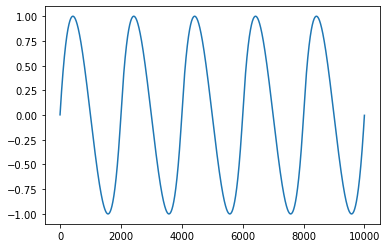
\includegraphics[width=0.75\textwidth]{10.png}
        \caption{Создание сигнала}
        \label{10}
\end{figure}

Дважды применим функцию \texttt{diff} и получи пилообразный сигнал, что довольно логично после выполнения предыдущего упражнения.

\begin{lstlisting}[caption= Применение \texttt{diff}]
out_wave = in_wave.diff().diff()
out_wave.plot()
\end{lstlisting}

\begin{figure}[H]
        \centering
        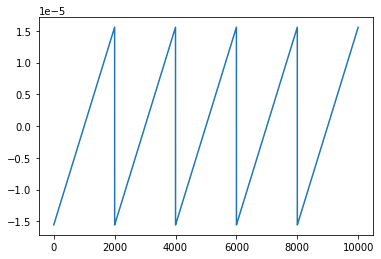
\includegraphics[width=0.75\textwidth]{11.png}
        \caption{Применение \texttt{diff}}
        \label{11}
\end{figure}



Когда мы дифференцируем дважды, получаем пилообразную форму с некоторым звоном. Проблема в том, что производная параболического сигнала в точках не определена.

\begin{lstlisting}[H]
spectrum = in_wave.make_spectrum().differentiate().differentiate()
out_wave2 = spectrum.make_wave()
out_wave2.plot()
\end{lstlisting}

\begin{figure}[H]
        \centering
        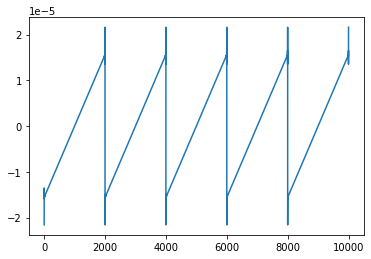
\includegraphics[width=0.75\textwidth]{12.png}
        \caption{}
        \label{12}
\end{figure}

В конце работы я вывел фильтры для второй разницы и второй производной фильтры и сравнил их:

Рассмотрим два фильтра в одном масштабе:

\begin{lstlisting}[caption=Визуализация двух фильтров]
diff_filter.plot(label='2nd diff')
deriv_filter.plot(label='2nd deriv')
\end{lstlisting}

\begin{figure}[H]
        \centering
        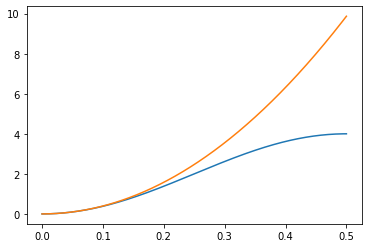
\includegraphics[width=0.75\textwidth]{13.png}
        \caption{Визуализация двух фильтров(синий - diff, оранжевый - deriv)}
        \label{13}
\end{figure}

Теперь мы можем видеть, что оба являются фильтрами верхних частот, которые усиливают компоненты самых высоких частот. Второй \texttt{deriv} параболический, поэтому он сильнее всего усиливает самые высокие частоты. Второй \texttt{diff} - хорошее приближение второй производной только на самых низких частотах, затем он существенно отклоняется.

\chapter{Выводы}

Во время выполнения лабораторной работы получены навыки работы с взаимосвязью между окнами во временной области и фильтрами в частотной области. Также изучалось влияние окна конечных разностей, которое приближает дифференцирование, и операции накопления суммы, которая приближает интегрирование.

\end{document}